\vspace{-2mm}
\section{Results}
\label{sec:results}

We discuss three key results related to (1) the rising use of web, social media and synthetic sources, (2) inconsistent and opaque restrictions on data use, and (3) a lack of improvement in geographical or linguistic representation.
Each of these findings holds across modalities, at the ecosystem level.

\vspace{-2mm}
\subsection{Rising Use of Web, Social Media \& Synthetic Data}
\label{sec:data-sources}

\begin{figure*}[!htb]
    \centering
    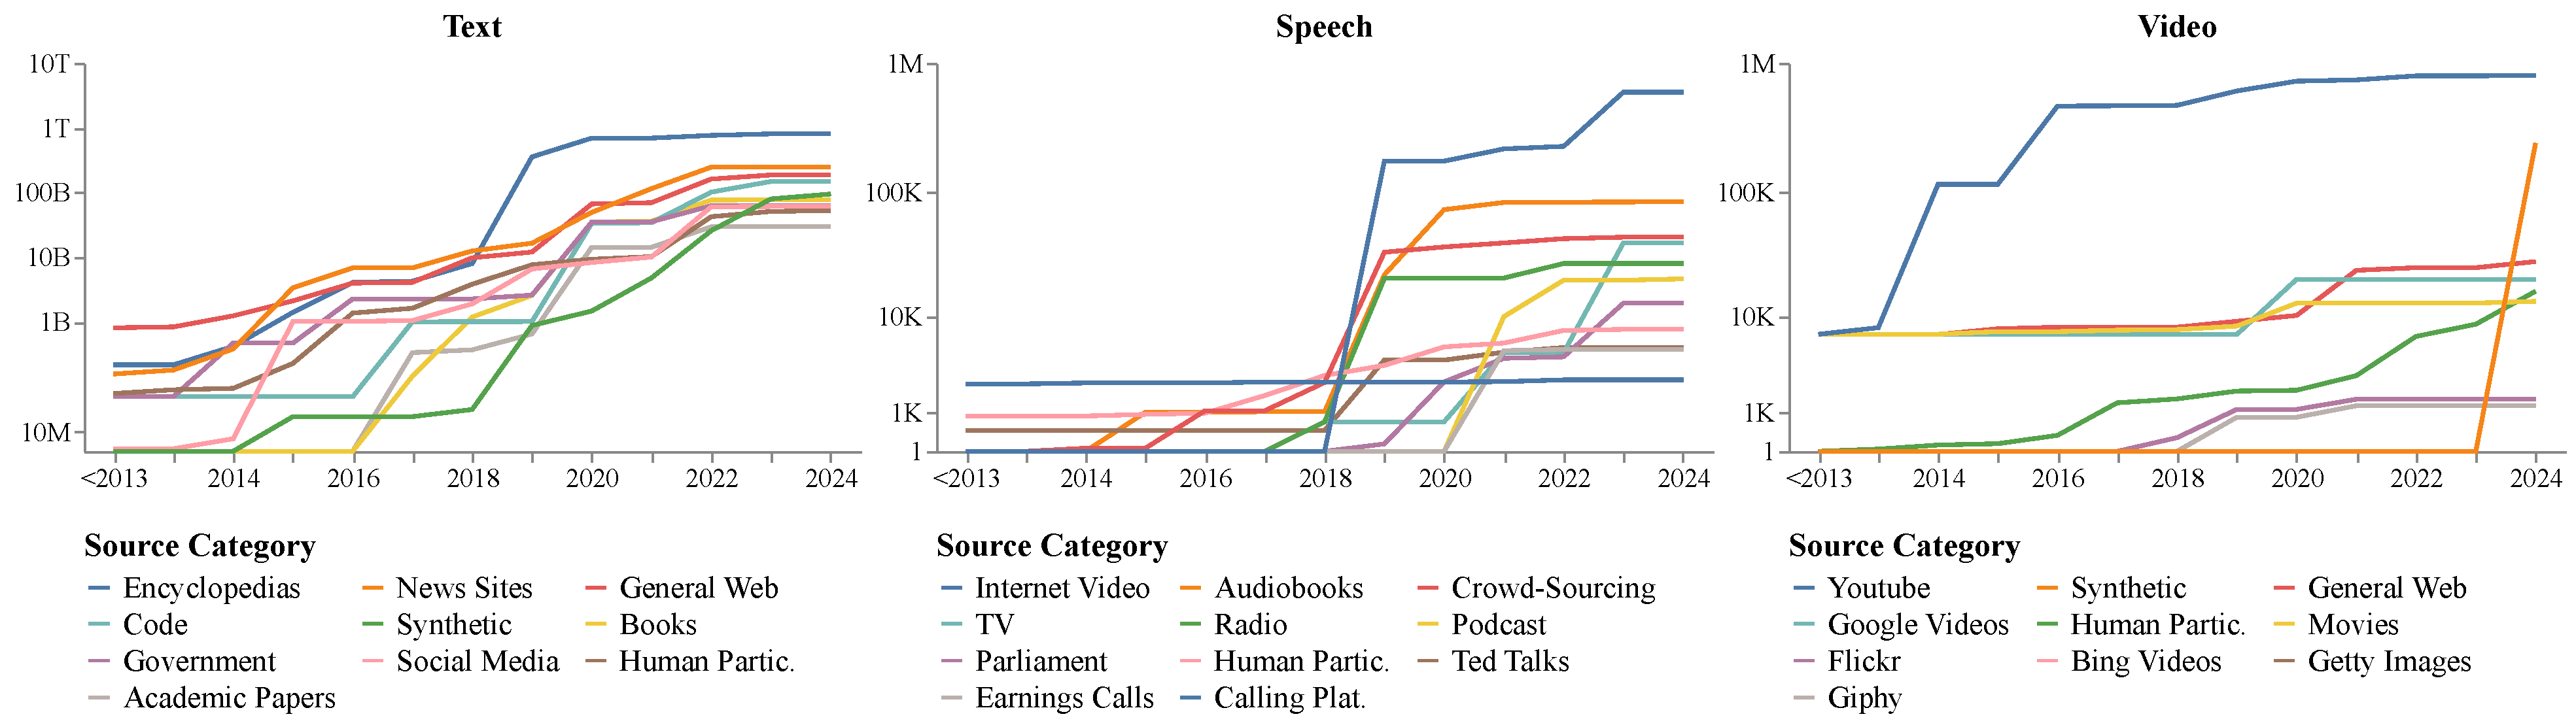
\includegraphics[width=\textwidth]{figures/temporal-sources-v2.pdf}
    \caption{The cumulative size of data (log-scale tokens for text, hours for speech/video) from each source category, across modalities. The source categories in the legend are ordered by descending quantity. \textbf{Speech and video sources are increasingly dominated by internet videos and YouTube. Whereas text is predominantly web or encyclopedia-based (wiki) sources, synthetic text is rising in popularity.} }
    \label{fig:temporal-source-categories}
    \vspace{-3mm}
\end{figure*}

\vspace{-2mm}
\paragraph{The need for scale, and heterogeneity have driven rising use of data from web-crawled, social media, and synthetic data sources.}
Developers have sought out ever larger and conveniently accessible sources of training data \citep{hoffmann2022training, henighan2020scalinglawsautoregressivegenerative}.
While small, human-curated datasets are often sufficient and sometimes preferred due to higher quality, these sources often do not scale to present demands \citep{kaplan2020scaling, henighan2020scalinglawsautoregressivegenerative}.
In \Cref{fig:temporal-source-categories}, we empirically measure the rising use of web crawling and social media (or ``forum'') websites that provide some of the most scalable and fresh content.
While web-sourced data was always prominent, the balance of sources becomes much more skewed after 2018---note the use of the y-axis log scale.
We find for Speech and Video that by far the most prominent source of data has become internet videos, and specifically YouTube. 
Nearly 1M hours each of Speech and Video data from this source far outstrips the next most common sources, which comprise less than 100K hours.
For Speech, the primary data sources used to be Calling Platforms (pre-2017), content manually collected with Human Participation, and Audiobooks, but since 2018 internet videos have supplanted these other sources.
For Video, since 2013, YouTube, synthetic, and general web data sources all constitute a significantly larger portion of data used in prominent video datasets, outstripping the use of Movies, Flickr, Getty, or human curated sources.
Among text post-training datasets, we see a similar trend with general or news web-based sources, including encyclopedic sources (mainly Wikipedia), providing the majority of tokens over time.
Encyclopedic sources alone now contribute over 1T tokens in total.

\paragraph{Synthetic data sources are rising the most rapidly.}
Within the video modality, the introduction of VidProm \citep{wang2024vidprom} in 2024, consisting of nearly 7M synthetically generated videos, offered a large shift in the video source distribution.
Within the textual modality, from \cref{fig:temporal-source-categories}, synthetic data represented <0.1\% of the quantity of Web Encyclopedia data in 2020, but is now 10\% its proportion in 2024, making up the 5th largest source of tokens.
% If we were to consider pretraining data sources, such as C4 \citep{raffel2020exploring}, or Dolma \citep{soldaini2024dolma}, then usually the web sources far exceed alternative sources such as books, government data, exams, academic papers, or expert curated sets.
The top models used in generating datasets are mainly from OpenAI. The top 5 consist of ChatGPT, version unspecified (15.0\% of synthetic datasets), GPT-4 (14.4\%), BART (10.1\%), GPT-3 (8.3\%) and GPT-3.5-Turbo (4.9\%). 
% Additionally, 15.2\% of datasets also used some kind of dataset-specific non-neural templating scheme.
The average synthetic dataset also has notably longer turns (in tokens) than the average natural dataset: 1,756 tokens vs 1,065.
The task distribution of textual synthetic datasets is shifted towards longer form, open-generation and creative tasks. For example, 88.1\% of natural datasets contain classification tasks, compared to only 66.3\% of synthetic datasets. Natural data is also more likely to cover translation than synthetic data (72.4\% of datasets vs only 22.9\% of synthetic datasets). 
% Both natural and synthetic datasets are mostly English-only, though synthetic datasets are slightly more likely to be English-only than natural datasets (76.3\% vs 69.6\%).



\begin{figure*}[htbp]
    \centering
    \begin{subfigure}[b]{0.99\textwidth}
        \centering
        % Replace with your first plot code
        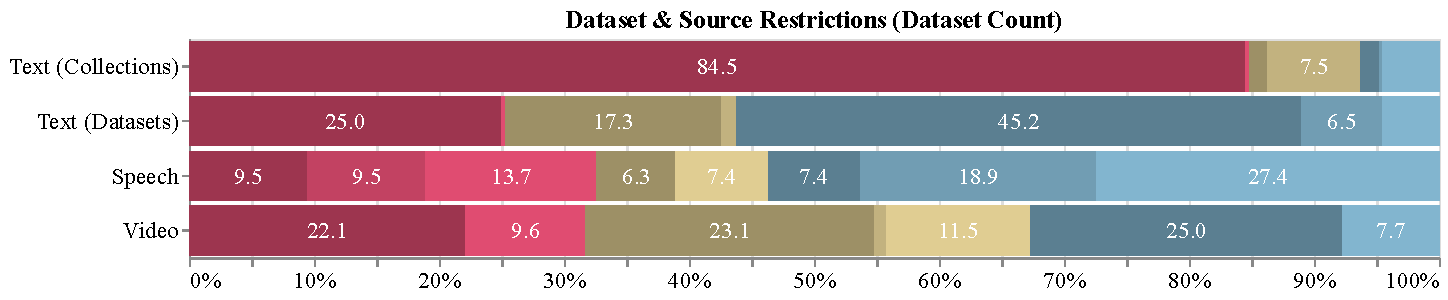
\includegraphics[width=\linewidth]{figures/license-terms-count.pdf} 
        % \caption{Total Language Representation}
    \end{subfigure}
    \vspace{0.3cm}
    \begin{subfigure}[b]{0.99\textwidth}
        \centering
        % Replace with your third plot code
        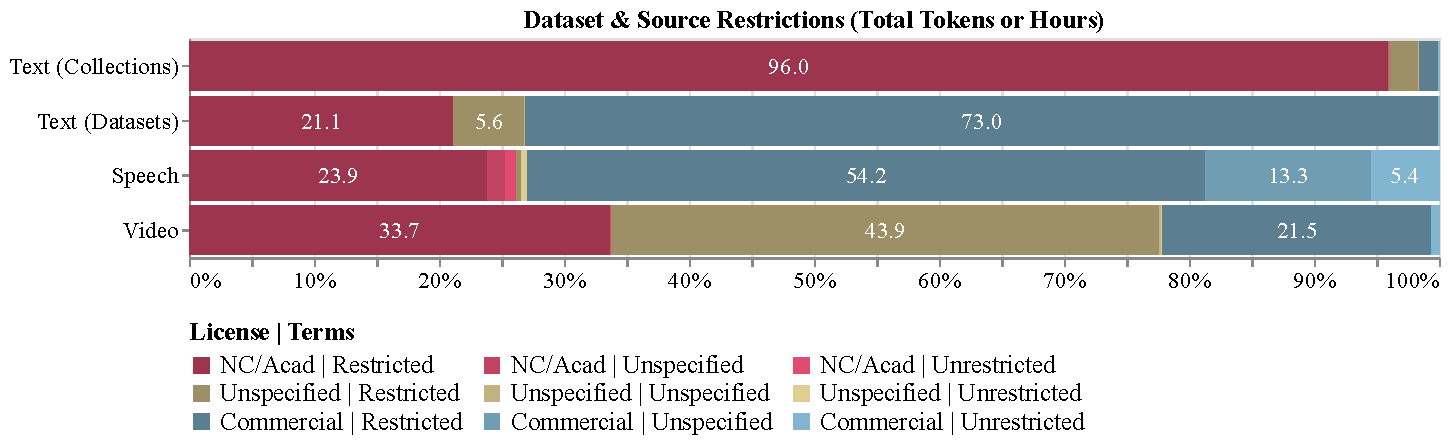
\includegraphics[width=\linewidth]{figures/license-terms-hours.pdf} 
        % \caption{Total Geographical Representation}
    \end{subfigure}
    \caption{The distribution of restrictions from dataset \emph{licenses} and their sources' \emph{terms}. We break this down by the count of datasets (top), as well as total tokens or hours (bottom). 
    Each license is categorized as Non-commercial/Academic (NC/Acad), Unspecified, or Commercially licensed.
    Each dataset may also have terms from the source: Restricted to non-commercial use, Unspecified restrictions, or Unrestricted.
    \textbf{Two main findings across modalities emerge: (1) Commercially licensed datasets represent a larger set of tokens and hours, relative to number of datasets; however, (2) the vast majority of those commercially licensed tokens/hours bare restrictions from their sources.}
    \Cref{tab:license_terms_breakdown,tab:license_terms_breakdown_count} in the appendix provide detailed numbers.}
    \label{fig:license-terms}
    \vspace{-3mm}
\end{figure*}


\vspace{-2mm}
\subsection{Inconsistent Use Restrictions}
\label{sec:use-restrictions}

In the United States, creators of a work automatically have a copyright interest that gives them exclusive rights to make copies and derivatives of the work (17 U.S.C. § 106). \emph{Licenses} are legal documents through which the owners of a work express how others may use their work. By contrast, \emph{Terms of Service} express a contract between a platform and its users to spell out how a platform and its content may be used~\citep{robinson2020beyond}.  
For simplicity, we use \emph{``Licenses''} to refer to dataset restrictions, and \emph{``Terms''} to refer to restrictions on the sources of datasets.
There remain open questions about whether certain data licenses are enforceable, but these licenses signal the intention of data creators and therefore warrant consideration as the data creators may be best positioned to understand the sensitivities of the data (privacy, copyright, representation, etc.), and the most impacted by its downstream use~\citep{morton2023licensed, lee2023talkin, mahari2023discit, mahari2023comment}.
The extent to which a practitioner adheres to dataset licenses or source terms remains an open question, and may depend on jurisdiction or the desired model's use cases \citep{lee2023talkin}. 
\emph{This work does not propose one standard for all developers.}
For these reasons we restrict our treatment and discussion here to tracing the lineage and distribution of licenses and terms for a given modality. 
    
\vspace{-2mm}
\paragraph{Data source terms are much more restrictive than the dataset's documented license restrictions.}
In \Cref{fig:license-terms}, we find only 25\%, 33\%, and 32\% of text/speech/video datasets are licensed non-commercially.
This value is even lower if we consider the proportion of tokens or hours, with 21\%, 26\%, and 33\% of text/speech/video quantities carrying license restrictions.
However, a staggering 99.8\%, 78\%, and 99\% of those quantities carry some form of non-commercial restriction on one of their sources.
For text, these restrictions are frequently from being generated by OpenAI or other models with a non-compete clause, while for speech and videos this is often since the datasets are derived from web or social media sources.

\vspace{-2mm}
\paragraph{Inconsistencies between dataset licenses and their source's restrictions pose challenges to practitioners.}
A large amount of datasets have permissive or unspecified licenses, but some set of their sources carry non-commercial restrictions.
This inconsistency is measurable---representing 79\% of tokens in text datasets, 55\% of speech hours, and 65\% of video hours.
Additionally, 19\%, 14\%, and 36\% of text, speech, and video datasets have no license or intended use documentation (from our audit of the datasets' documentation on Hugging Face Datasets, GitHub, and Papers with Code).
A lack of centralized documentation around these restrictions means it can be misleading to developers who are attempting to source data according to their own legal standards for copyright and privacy.
Furthermore, lack of documentation can hamper developers following best practices around data preparation and transparency \citep{gebru2021datasheets, bommasani2023foundation}.

\vspace{-2mm}
\paragraph{Large quantities of commercially licensed text datasets are locked in collections without clear information to separate them from restrictive datasets.}
% \paragraph{Text collections package restricted and unrestricted datasets, without clear information to separate them.}
In \Cref{fig:license-terms} (top and bottom), we see the number of datasets and number of tokens \emph{without} restrictions is significantly higher for Text (Datasets) than Text (Collections).
Specifically, 60\% more Datasets (or 75\% more tokens) are commercially licensed, than for Collections.
This demonstrates that many collections contain significant amounts of commercially licensed data.
While our audit traces licenses for all datasets within a collection, most collections do not aggregate or expose this documentation.
As a result, practitioners may be left without easy access to filter for the  subsets appropriate for their sourcing standards.

\vspace{-2mm}
\subsection{Geographical \& Linguistic Representation is Not Improving}
\label{sec:representation}

\begin{figure*}[!ht]
  \centering
  \begin{minipage}{0.99\textwidth}
    \centering
    \includegraphics[width=\textwidth]{figures/globes-v3.pdf}
  \end{minipage}\hfill
  \begin{minipage}{0.99\textwidth}
    \centering
    \begin{tabular}{l|cccccc}
        \toprule
         & \textsc{Africa} & \textsc{Asia} & \textsc{Europe} & \textsc{N America} & \textsc{Oceania} & \textsc{S America} \\
        \midrule
        \multicolumn{7}{c}{\textbf{\emph{By Count}}} \\
        \midrule
        \textsc{Text} & 0.3 & 13.4 & 24.0 & 61.5 & 0.7 & 0.2 \\
        \textsc{Speech} & 3.6 & 35.7 & 30.4 & 30.4 & 0.0 & 0.0 \\
        \textsc{Video} & 0.0 & 25.2 & 24.4 & 48.0 & 0.8 & 1.6 \\
        \midrule
        \multicolumn{7}{c}{\textbf{\emph{By Tokens or Hours}}} \\
        \midrule
        \textsc{Text} & 0.0 & 6.1 & 55.4 & 38.4 & 0.1 & 0.0 \\
        \textsc{Speech} & 0.1 & 38.8 & 18.8 & 42.4 & 0.0 & 0.0 \\
        \textsc{Video} & 0.0 & 23.1 & 22.0 & 38.2 & 16.7 & 0.1 \\
        \bottomrule
    \end{tabular}
  \end{minipage}
  \vspace{1mm}
  \caption{The geographical distribution of countries (world maps) and continents (table) represented by dataset creators. \textbf{Despite some differences in European, Russian, and Middle Eastern representation, creators are heavily concentrated in the US, China, and  Western Europe, with little to no representation in South America or Africa, across modalities.} The current Gini coefficient for (Text, Speech, Video) = (0.92, 0.86, 0.74), where higher values indicate more concentration.}
  \label{fig:creator-worldmaps}
  \vspace{-3mm}
\end{figure*}

\vspace{-2mm}
\paragraph{The importance and progress of representation in AI training data.}
Diversity and representation in training datasets, and among their creators, are widely acknowledged as essential to building AI models that are less biased, more useful, and more equitable \citep{joshi2020state,singh2024aya,ustun2024aya,adelani2021masakhaner,adelani2024irokobenchnewbenchmarkafrican,aakanksha2024multilingualalignmentprismaligning, mcmillanmajor2022documentinggeographicallycontextuallydiverse, porgali2023casualconversationsv2dataset, monfort2019moments, sigurdsson2016hollywoodhomescrowdsourcingdata}.
Prior work has measured the diversity of languages in data along with cultural, ideological, and geographical imbalances \citep{faisal2022dataset,shankar2017no,mcmillan2022documenting,de2019does,mahadev2021understanding}.
These studies have exposed significant flaws, often in the form of bias and discrimination, stemming directly from poor representation in data \citep{buolamwiniGenderShades2018, birhane2021multimodal}.
As this problem has now been widely acknowledged for decades, recent efforts have foregrounded sourcing data multilingually and multi-culturally, from native speakers and creators (e.g. ROOTS \citep{NEURIPS2022_ce9e92e3}, the Aya Dataset \citep{singh2024aya}, the SEACrowd Catalogue \citep{lovenia2024seacrowd}, the Masader Catalogue \citep{alyafeai2022masader}, Common Voice \citep{ardila2019common}, Causal Conversations V2 \citep{porgali2023casualconversationsv2dataset} or Moments in Time \citep{monfort2019moments}).

\vspace{-2mm}
\paragraph{Measuring geographical and linguistic representation.}
Naturally, we aim to use our audit to measure the progress of these efforts on geographical and linguistic representation in the AI ecosystem.
We measure the progress of two forms of representation: (1) language diversity of text and speech data, and (2) geographical diversity of the creators, in all three modalities.
For languages, we use the ISO 639-1 and 639-3 language codes and categories of language families from Glottolog 5.0.\footnote{We use top level \href{https://glottolog.org/}{Glottolog} families.}
In \Cref{fig:representation}(a, c) we display the cumulative sum of unique languages and countries present across all audited datasets, at each time period since 2013.
While these measurements illustrate the absolute rise in diversity, we also hope to measure the relative dispersion, or equality of languages and countries in the distribution.
In \Cref{fig:representation}(b, d), we use the Gini Index \citep{e7461144-3bdb-3344-8d83-b11a52be7f2f, atkinson1970measurement}, a traditional measure of statistical dispersion, frequently used to quantify inequality.
This allows us to understand if the distributions of languages and creators are more representative of the international community over the last decade, or equally concentrated despite apparent efforts at the margins.

\vspace{-2mm}
\paragraph{Inequality in geographical representation remains very high, with few organizations creating datasets from the Global South.}
For every dataset, our audit recorded the organizational affiliations of each creator of the dataset.\footnote{A dataset creator, following \citep{longpre2023data}, is defined as an organization associated with the release of the dataset as created for machine learning---not any of the upstream sources. More details in \Cref{app:datasets}.}
These organizations were then manually mapped to the country in which they are headquartered. 
Occasionally, organizations like BigScience, BigCode, or Masakhane have international or continental representation, and were counted as such.
In \Cref{fig:creator-worldmaps}, we measure the current state of diversity among these creator organizations---where a Gini coefficient of 1 indicates highest concentration, and lower values more broad representation.
Without taking up the normative question of what a truly ``fair'' score would be, these values provide useful comparisons across modalities and over time.
We find that Text dataset developers are particularly homogeneous, with a Gini-coefficient of 0.92; followed by Speech, at 0.86 and Video at 0.74, which remain high, but are meaningfully less concentrated. \Cref{fig:creator-worldmaps} also illustrates that even this limited diversity is still concentrated in North America, Europe, East Asia, and less so in the Global South.

In \Cref{fig:creator-worldmaps}, we also compare the distribution of datasets, and of tokens or hours by continent. 
Dataset creators affiliated with African or South American organizations account for fewer than 0.2\% of all tokens or hours, in each modality.
In contrast, Asian affiliated organizations represent large proportions of the data, particularly for speech (39\% of hours, attributed predominantly to YODAS \citep{li2023yodas}).
Much of this driven by Chinese, Indian, Russian, and Saudi Arabian creators.
Most prominently, the combination of North American and European datasets comprises 93\% of text tokens, 61\% of speech hours, and 60\% of video hours.

\begin{figure*}[htbp]
    \centering
    \begin{subfigure}[b]{0.49\textwidth}
        \centering
        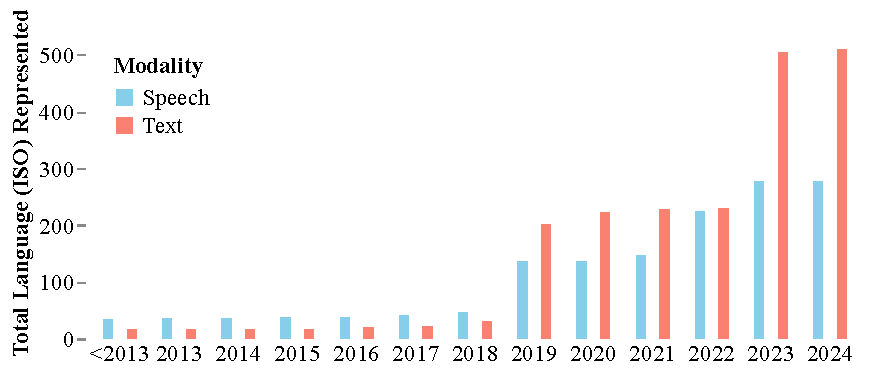
\includegraphics[width=\linewidth]{figures/temporal-cumulative-languages.pdf} 
        \caption{Total Language Representation}
    \end{subfigure}
    \hfill
    \begin{subfigure}[b]{0.49\textwidth}
        \centering
        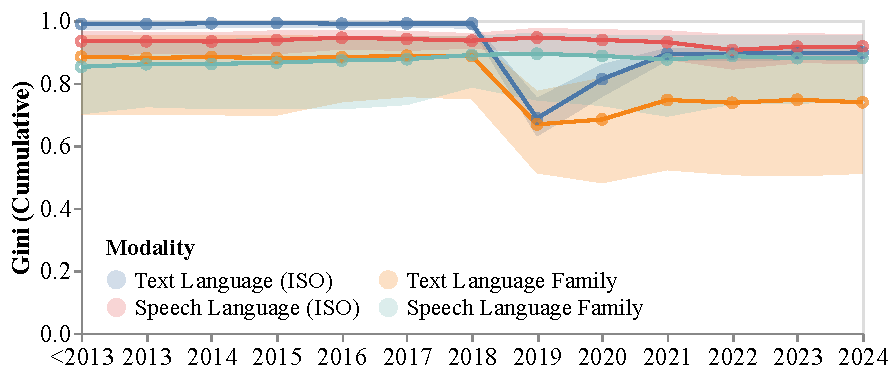
\includegraphics[width=\linewidth]{figures/temporal-language-gini.pdf} 
        \caption{Gini-coefficient for Language Representation}
    \end{subfigure}

    \vspace{0.3cm}

    \begin{subfigure}[b]{0.49\textwidth}
        \centering
        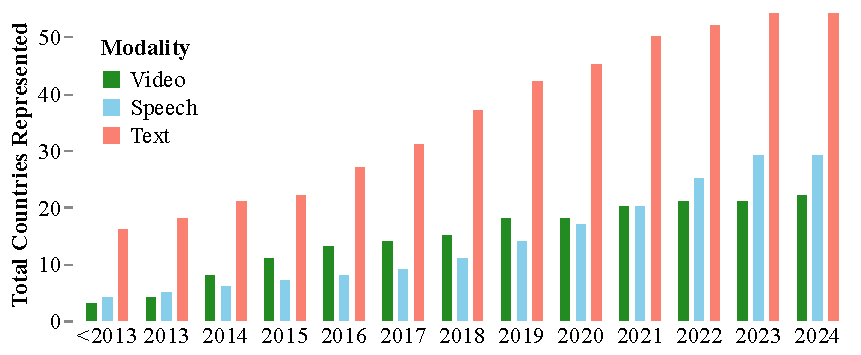
\includegraphics[width=\linewidth]{figures/temporal-cumulative-geo.pdf} 
        \caption{Total Geographical Representation}
    \end{subfigure}
    \hfill
    \begin{subfigure}[b]{0.49\textwidth}
        \centering
        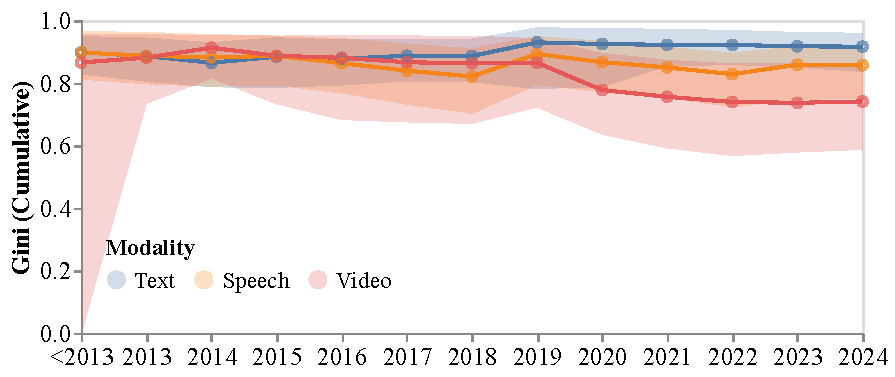
\includegraphics[width=\linewidth]{figures/temporal-geo-gini.pdf} 
        \caption{Gini-coefficient for Geographical Representation}
    \end{subfigure}
    
    \caption{The cumulative totals (left) of languages and countries represented in the data over time, and the 95\% confidence intervals of the gini-coefficients over time (right) to measure the representativeness of these variables. Gini-coefficients are a measure of statistical dispersion, frequently used to quantify inequality. 
    A Gini coefficient of 1 indicates highest concentration, and lower values more broad representation.
    \textbf{While the number of represented languages and geographies continue to rise (left), the equality of their distribution has in most cases, not significantly changed.} 
    }
    \label{fig:representation}
\end{figure*}

\vspace{-2mm}
\paragraph{Geographical representation has not significantly improved for over a decade.}
In \Cref{fig:representation}(c), we measure the total unique number of countries represented across all dataset creator organizations. While individual creators will have varying ethnic and national affiliation, we treat this as an estimate for the influence of each locale in dataset development. We find that while the number of represented countries has risen steadily each year, for each modality, this represents only an illusion of progress. Empirically, the Gini coefficient for each modality has not significantly changed since the start of the period we examine in 2013. Geographic diversity has increased only among Video datasets, and these increases are not significant at the $p = 0.05$ level. Text and Speech geographical representations appear to remain stable over the last decade of AI development.

\vspace{-2mm}
\paragraph{Multilingual representation has not improved by most measures.}
Similar to geographical representation, we measure the cumulative number of ISO 639-1 languages and language families over time, as well as the per-modality Gini-coefficient.
\Cref{fig:representation}(a) shows significant increases in the number of languages available for speech and text, especially in 2019, and 2023, with the introduction of large sets like Flores \citep{goyal2022flores}, xP3x \citep{muennighoff2023crosslingual}, Common Voice \citep{ardila2019common}, and the Aya Collection \citep{singh2024aya}. However, once again, when measuring the cumulative dispersion of these datasets in \Cref{fig:representation}(b), only Text language families demonstrate any improvement from pre-2013 to the present. Improvements in the Gini coefficient appear to be largely driven by individual large-scale projects like xP3x and Common Voice, both introduced in 2019. Subsequently, newer datasets remain predominantly monolingual, causing measures of concentration in text languages, speech languages, and language families to remain consistently high.

\begin{figure*}[!htb]
    \centering
    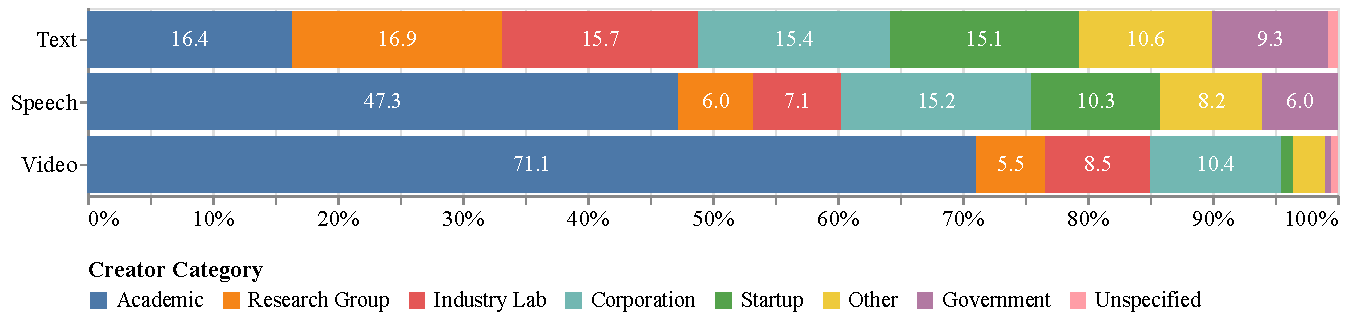
\includegraphics[width=\textwidth]{figures/creator_categories_by_modality.pdf}
    \caption{The distribution of creator organizations by modality. \textbf{Most public speech and video datasets are developed by academic organizations, whereas text datasets are developed by a wide mix of academia, non-profit or industry labs, as well as startups.} 
    }
    \label{fig:creator-orgs}
    \vspace{-3mm}
\end{figure*}

\vspace{-2mm}
\paragraph{Academia, research non-profits, and industry labs continue to drive public dataset development.}
As well as understanding the geographic associations of the organizations creating popular datasets, we manually categorize them into: Academic Organization (e.g., universities), Research Groups (e.g., non-profits such as BigScience, EleutherAI or AI2), Industry Labs (e.g., Cohere For AI, Google DeepMind), Corporations (e.g. Google, Meta), Startups (e.g., OpenAI, Anthropic), Governments, Unspecified (datasets where owner affiliation is not shared), or Other.
When a dataset is released in collaboration between organizations, we record each organization.
In \Cref{fig:creator-orgs}, we find that universities and other academic organizations account for 16\%, 47\%, and 71\% of all recorded dataset releases, across Text, Speech, and Video respectively.
Research groups, industry labs and even corporations are also significant contributors, especially for Text datasets, where ecosystem contributors are far more distributed.
The significant role of academic organizations in Video and Speech may suggest that the risk profile of releasing Text datasets differs somewhat from Video and Speech datasets, which may have more distinct privacy concerns.